% Created by tikzDevice version 0.12.3.1 on 2022-11-21 12:04:03
% !TEX encoding = UTF-8 Unicode
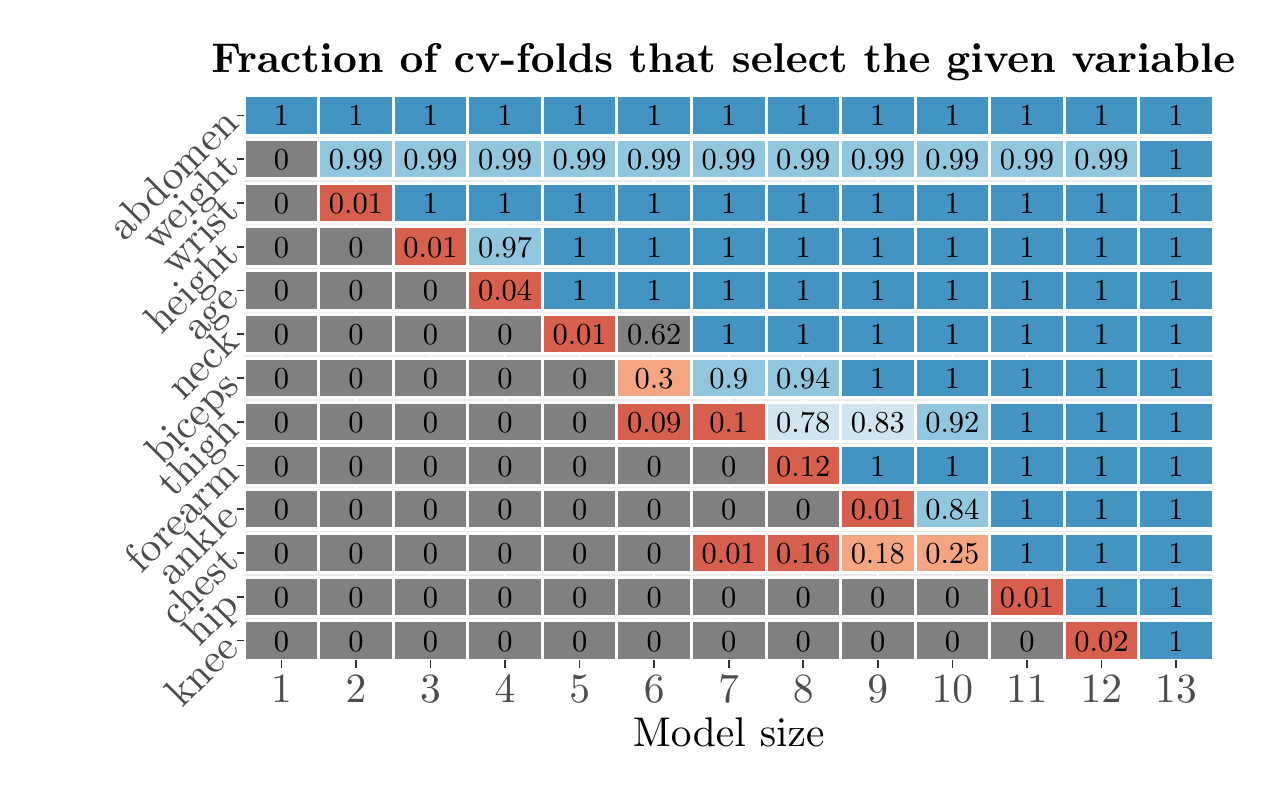
\begin{tikzpicture}[x=1pt,y=1pt]
\definecolor{fillColor}{RGB}{255,255,255}
\begin{scope}
\definecolor{drawColor}{RGB}{255,255,255}
\definecolor{fillColor}{RGB}{255,255,255}

\path[draw=drawColor,line width= 0.6pt,line join=round,line cap=round,fill=fillColor] (  0.00,  0.00) rectangle (433.62,268.00);
\end{scope}
\begin{scope}
\definecolor{fillColor}{gray}{0.92}

\path[fill=fillColor] ( 77.94, 39.69) rectangle (428.12,243.73);
\definecolor{drawColor}{RGB}{255,255,255}

\path[draw=drawColor,line width= 0.6pt,line join=round] ( 77.94, 46.81) --
	(428.12, 46.81);

\path[draw=drawColor,line width= 0.6pt,line join=round] ( 77.94, 62.63) --
	(428.12, 62.63);

\path[draw=drawColor,line width= 0.6pt,line join=round] ( 77.94, 78.44) --
	(428.12, 78.44);

\path[draw=drawColor,line width= 0.6pt,line join=round] ( 77.94, 94.26) --
	(428.12, 94.26);

\path[draw=drawColor,line width= 0.6pt,line join=round] ( 77.94,110.08) --
	(428.12,110.08);

\path[draw=drawColor,line width= 0.6pt,line join=round] ( 77.94,125.89) --
	(428.12,125.89);

\path[draw=drawColor,line width= 0.6pt,line join=round] ( 77.94,141.71) --
	(428.12,141.71);

\path[draw=drawColor,line width= 0.6pt,line join=round] ( 77.94,157.53) --
	(428.12,157.53);

\path[draw=drawColor,line width= 0.6pt,line join=round] ( 77.94,173.35) --
	(428.12,173.35);

\path[draw=drawColor,line width= 0.6pt,line join=round] ( 77.94,189.16) --
	(428.12,189.16);

\path[draw=drawColor,line width= 0.6pt,line join=round] ( 77.94,204.98) --
	(428.12,204.98);

\path[draw=drawColor,line width= 0.6pt,line join=round] ( 77.94,220.80) --
	(428.12,220.80);

\path[draw=drawColor,line width= 0.6pt,line join=round] ( 77.94,236.61) --
	(428.12,236.61);

\path[draw=drawColor,line width= 0.6pt,line join=round] ( 91.40, 39.69) --
	( 91.40,243.73);

\path[draw=drawColor,line width= 0.6pt,line join=round] (118.34, 39.69) --
	(118.34,243.73);

\path[draw=drawColor,line width= 0.6pt,line join=round] (145.28, 39.69) --
	(145.28,243.73);

\path[draw=drawColor,line width= 0.6pt,line join=round] (172.22, 39.69) --
	(172.22,243.73);

\path[draw=drawColor,line width= 0.6pt,line join=round] (199.15, 39.69) --
	(199.15,243.73);

\path[draw=drawColor,line width= 0.6pt,line join=round] (226.09, 39.69) --
	(226.09,243.73);

\path[draw=drawColor,line width= 0.6pt,line join=round] (253.03, 39.69) --
	(253.03,243.73);

\path[draw=drawColor,line width= 0.6pt,line join=round] (279.96, 39.69) --
	(279.96,243.73);

\path[draw=drawColor,line width= 0.6pt,line join=round] (306.90, 39.69) --
	(306.90,243.73);

\path[draw=drawColor,line width= 0.6pt,line join=round] (333.84, 39.69) --
	(333.84,243.73);

\path[draw=drawColor,line width= 0.6pt,line join=round] (360.78, 39.69) --
	(360.78,243.73);

\path[draw=drawColor,line width= 0.6pt,line join=round] (387.71, 39.69) --
	(387.71,243.73);

\path[draw=drawColor,line width= 0.6pt,line join=round] (414.65, 39.69) --
	(414.65,243.73);
\definecolor{fillColor}{RGB}{67,147,195}

\path[draw=drawColor,line width= 1.1pt,fill=fillColor] ( 77.94,229.49) rectangle (104.87,243.73);

\path[draw=drawColor,line width= 1.1pt,fill=fillColor] (104.87,229.49) rectangle (131.81,243.73);

\path[draw=drawColor,line width= 1.1pt,fill=fillColor] (131.81,229.49) rectangle (158.75,243.73);

\path[draw=drawColor,line width= 1.1pt,fill=fillColor] (158.75,229.49) rectangle (185.68,243.73);

\path[draw=drawColor,line width= 1.1pt,fill=fillColor] (185.68,229.49) rectangle (212.62,243.73);

\path[draw=drawColor,line width= 1.1pt,fill=fillColor] (212.62,229.49) rectangle (239.56,243.73);

\path[draw=drawColor,line width= 1.1pt,fill=fillColor] (239.56,229.49) rectangle (266.50,243.73);

\path[draw=drawColor,line width= 1.1pt,fill=fillColor] (266.50,229.49) rectangle (293.43,243.73);

\path[draw=drawColor,line width= 1.1pt,fill=fillColor] (293.43,229.49) rectangle (320.37,243.73);

\path[draw=drawColor,line width= 1.1pt,fill=fillColor] (320.37,229.49) rectangle (347.31,243.73);

\path[draw=drawColor,line width= 1.1pt,fill=fillColor] (347.31,229.49) rectangle (374.25,243.73);

\path[draw=drawColor,line width= 1.1pt,fill=fillColor] (374.25,229.49) rectangle (401.18,243.73);

\path[draw=drawColor,line width= 1.1pt,fill=fillColor] (401.18,229.49) rectangle (428.12,243.73);
\definecolor{fillColor}{gray}{0.50}

\path[draw=drawColor,line width= 1.1pt,fill=fillColor] ( 77.94,213.68) rectangle (104.87,227.91);
\definecolor{fillColor}{RGB}{146,197,222}

\path[draw=drawColor,line width= 1.1pt,fill=fillColor] (104.87,213.68) rectangle (131.81,227.91);

\path[draw=drawColor,line width= 1.1pt,fill=fillColor] (131.81,213.68) rectangle (158.75,227.91);

\path[draw=drawColor,line width= 1.1pt,fill=fillColor] (158.75,213.68) rectangle (185.68,227.91);

\path[draw=drawColor,line width= 1.1pt,fill=fillColor] (185.68,213.68) rectangle (212.62,227.91);

\path[draw=drawColor,line width= 1.1pt,fill=fillColor] (212.62,213.68) rectangle (239.56,227.91);

\path[draw=drawColor,line width= 1.1pt,fill=fillColor] (239.56,213.68) rectangle (266.50,227.91);

\path[draw=drawColor,line width= 1.1pt,fill=fillColor] (266.50,213.68) rectangle (293.43,227.91);

\path[draw=drawColor,line width= 1.1pt,fill=fillColor] (293.43,213.68) rectangle (320.37,227.91);

\path[draw=drawColor,line width= 1.1pt,fill=fillColor] (320.37,213.68) rectangle (347.31,227.91);

\path[draw=drawColor,line width= 1.1pt,fill=fillColor] (347.31,213.68) rectangle (374.25,227.91);

\path[draw=drawColor,line width= 1.1pt,fill=fillColor] (374.25,213.68) rectangle (401.18,227.91);
\definecolor{fillColor}{RGB}{67,147,195}

\path[draw=drawColor,line width= 1.1pt,fill=fillColor] (401.18,213.68) rectangle (428.12,227.91);
\definecolor{fillColor}{gray}{0.50}

\path[draw=drawColor,line width= 1.1pt,fill=fillColor] ( 77.94,197.86) rectangle (104.87,212.10);
\definecolor{fillColor}{RGB}{214,96,77}

\path[draw=drawColor,line width= 1.1pt,fill=fillColor] (104.87,197.86) rectangle (131.81,212.10);
\definecolor{fillColor}{RGB}{67,147,195}

\path[draw=drawColor,line width= 1.1pt,fill=fillColor] (131.81,197.86) rectangle (158.75,212.10);

\path[draw=drawColor,line width= 1.1pt,fill=fillColor] (158.75,197.86) rectangle (185.68,212.10);

\path[draw=drawColor,line width= 1.1pt,fill=fillColor] (185.68,197.86) rectangle (212.62,212.10);

\path[draw=drawColor,line width= 1.1pt,fill=fillColor] (212.62,197.86) rectangle (239.56,212.10);

\path[draw=drawColor,line width= 1.1pt,fill=fillColor] (239.56,197.86) rectangle (266.50,212.10);

\path[draw=drawColor,line width= 1.1pt,fill=fillColor] (266.50,197.86) rectangle (293.43,212.10);

\path[draw=drawColor,line width= 1.1pt,fill=fillColor] (293.43,197.86) rectangle (320.37,212.10);

\path[draw=drawColor,line width= 1.1pt,fill=fillColor] (320.37,197.86) rectangle (347.31,212.10);

\path[draw=drawColor,line width= 1.1pt,fill=fillColor] (347.31,197.86) rectangle (374.25,212.10);

\path[draw=drawColor,line width= 1.1pt,fill=fillColor] (374.25,197.86) rectangle (401.18,212.10);

\path[draw=drawColor,line width= 1.1pt,fill=fillColor] (401.18,197.86) rectangle (428.12,212.10);
\definecolor{fillColor}{gray}{0.50}

\path[draw=drawColor,line width= 1.1pt,fill=fillColor] ( 77.94,182.04) rectangle (104.87,196.28);

\path[draw=drawColor,line width= 1.1pt,fill=fillColor] (104.87,182.04) rectangle (131.81,196.28);
\definecolor{fillColor}{RGB}{214,96,77}

\path[draw=drawColor,line width= 1.1pt,fill=fillColor] (131.81,182.04) rectangle (158.75,196.28);
\definecolor{fillColor}{RGB}{146,197,222}

\path[draw=drawColor,line width= 1.1pt,fill=fillColor] (158.75,182.04) rectangle (185.68,196.28);
\definecolor{fillColor}{RGB}{67,147,195}

\path[draw=drawColor,line width= 1.1pt,fill=fillColor] (185.68,182.04) rectangle (212.62,196.28);

\path[draw=drawColor,line width= 1.1pt,fill=fillColor] (212.62,182.04) rectangle (239.56,196.28);

\path[draw=drawColor,line width= 1.1pt,fill=fillColor] (239.56,182.04) rectangle (266.50,196.28);

\path[draw=drawColor,line width= 1.1pt,fill=fillColor] (266.50,182.04) rectangle (293.43,196.28);

\path[draw=drawColor,line width= 1.1pt,fill=fillColor] (293.43,182.04) rectangle (320.37,196.28);

\path[draw=drawColor,line width= 1.1pt,fill=fillColor] (320.37,182.04) rectangle (347.31,196.28);

\path[draw=drawColor,line width= 1.1pt,fill=fillColor] (347.31,182.04) rectangle (374.25,196.28);

\path[draw=drawColor,line width= 1.1pt,fill=fillColor] (374.25,182.04) rectangle (401.18,196.28);

\path[draw=drawColor,line width= 1.1pt,fill=fillColor] (401.18,182.04) rectangle (428.12,196.28);
\definecolor{fillColor}{gray}{0.50}

\path[draw=drawColor,line width= 1.1pt,fill=fillColor] ( 77.94,166.23) rectangle (104.87,180.46);

\path[draw=drawColor,line width= 1.1pt,fill=fillColor] (104.87,166.23) rectangle (131.81,180.46);

\path[draw=drawColor,line width= 1.1pt,fill=fillColor] (131.81,166.23) rectangle (158.75,180.46);
\definecolor{fillColor}{RGB}{214,96,77}

\path[draw=drawColor,line width= 1.1pt,fill=fillColor] (158.75,166.23) rectangle (185.68,180.46);
\definecolor{fillColor}{RGB}{67,147,195}

\path[draw=drawColor,line width= 1.1pt,fill=fillColor] (185.68,166.23) rectangle (212.62,180.46);

\path[draw=drawColor,line width= 1.1pt,fill=fillColor] (212.62,166.23) rectangle (239.56,180.46);

\path[draw=drawColor,line width= 1.1pt,fill=fillColor] (239.56,166.23) rectangle (266.50,180.46);

\path[draw=drawColor,line width= 1.1pt,fill=fillColor] (266.50,166.23) rectangle (293.43,180.46);

\path[draw=drawColor,line width= 1.1pt,fill=fillColor] (293.43,166.23) rectangle (320.37,180.46);

\path[draw=drawColor,line width= 1.1pt,fill=fillColor] (320.37,166.23) rectangle (347.31,180.46);

\path[draw=drawColor,line width= 1.1pt,fill=fillColor] (347.31,166.23) rectangle (374.25,180.46);

\path[draw=drawColor,line width= 1.1pt,fill=fillColor] (374.25,166.23) rectangle (401.18,180.46);

\path[draw=drawColor,line width= 1.1pt,fill=fillColor] (401.18,166.23) rectangle (428.12,180.46);
\definecolor{fillColor}{gray}{0.50}

\path[draw=drawColor,line width= 1.1pt,fill=fillColor] ( 77.94,150.41) rectangle (104.87,164.65);

\path[draw=drawColor,line width= 1.1pt,fill=fillColor] (104.87,150.41) rectangle (131.81,164.65);

\path[draw=drawColor,line width= 1.1pt,fill=fillColor] (131.81,150.41) rectangle (158.75,164.65);

\path[draw=drawColor,line width= 1.1pt,fill=fillColor] (158.75,150.41) rectangle (185.68,164.65);
\definecolor{fillColor}{RGB}{214,96,77}

\path[draw=drawColor,line width= 1.1pt,fill=fillColor] (185.68,150.41) rectangle (212.62,164.65);
\definecolor{fillColor}{gray}{0.50}

\path[draw=drawColor,line width= 1.1pt,fill=fillColor] (212.62,150.41) rectangle (239.56,164.65);
\definecolor{fillColor}{RGB}{67,147,195}

\path[draw=drawColor,line width= 1.1pt,fill=fillColor] (239.56,150.41) rectangle (266.50,164.65);

\path[draw=drawColor,line width= 1.1pt,fill=fillColor] (266.50,150.41) rectangle (293.43,164.65);

\path[draw=drawColor,line width= 1.1pt,fill=fillColor] (293.43,150.41) rectangle (320.37,164.65);

\path[draw=drawColor,line width= 1.1pt,fill=fillColor] (320.37,150.41) rectangle (347.31,164.65);

\path[draw=drawColor,line width= 1.1pt,fill=fillColor] (347.31,150.41) rectangle (374.25,164.65);

\path[draw=drawColor,line width= 1.1pt,fill=fillColor] (374.25,150.41) rectangle (401.18,164.65);

\path[draw=drawColor,line width= 1.1pt,fill=fillColor] (401.18,150.41) rectangle (428.12,164.65);
\definecolor{fillColor}{gray}{0.50}

\path[draw=drawColor,line width= 1.1pt,fill=fillColor] ( 77.94,134.59) rectangle (104.87,148.83);

\path[draw=drawColor,line width= 1.1pt,fill=fillColor] (104.87,134.59) rectangle (131.81,148.83);

\path[draw=drawColor,line width= 1.1pt,fill=fillColor] (131.81,134.59) rectangle (158.75,148.83);

\path[draw=drawColor,line width= 1.1pt,fill=fillColor] (158.75,134.59) rectangle (185.68,148.83);

\path[draw=drawColor,line width= 1.1pt,fill=fillColor] (185.68,134.59) rectangle (212.62,148.83);
\definecolor{fillColor}{RGB}{244,165,130}

\path[draw=drawColor,line width= 1.1pt,fill=fillColor] (212.62,134.59) rectangle (239.56,148.83);
\definecolor{fillColor}{RGB}{146,197,222}

\path[draw=drawColor,line width= 1.1pt,fill=fillColor] (239.56,134.59) rectangle (266.50,148.83);

\path[draw=drawColor,line width= 1.1pt,fill=fillColor] (266.50,134.59) rectangle (293.43,148.83);
\definecolor{fillColor}{RGB}{67,147,195}

\path[draw=drawColor,line width= 1.1pt,fill=fillColor] (293.43,134.59) rectangle (320.37,148.83);

\path[draw=drawColor,line width= 1.1pt,fill=fillColor] (320.37,134.59) rectangle (347.31,148.83);

\path[draw=drawColor,line width= 1.1pt,fill=fillColor] (347.31,134.59) rectangle (374.25,148.83);

\path[draw=drawColor,line width= 1.1pt,fill=fillColor] (374.25,134.59) rectangle (401.18,148.83);

\path[draw=drawColor,line width= 1.1pt,fill=fillColor] (401.18,134.59) rectangle (428.12,148.83);
\definecolor{fillColor}{gray}{0.50}

\path[draw=drawColor,line width= 1.1pt,fill=fillColor] ( 77.94,118.78) rectangle (104.87,133.01);

\path[draw=drawColor,line width= 1.1pt,fill=fillColor] (104.87,118.78) rectangle (131.81,133.01);

\path[draw=drawColor,line width= 1.1pt,fill=fillColor] (131.81,118.78) rectangle (158.75,133.01);

\path[draw=drawColor,line width= 1.1pt,fill=fillColor] (158.75,118.78) rectangle (185.68,133.01);

\path[draw=drawColor,line width= 1.1pt,fill=fillColor] (185.68,118.78) rectangle (212.62,133.01);
\definecolor{fillColor}{RGB}{214,96,77}

\path[draw=drawColor,line width= 1.1pt,fill=fillColor] (212.62,118.78) rectangle (239.56,133.01);

\path[draw=drawColor,line width= 1.1pt,fill=fillColor] (239.56,118.78) rectangle (266.50,133.01);
\definecolor{fillColor}{RGB}{209,229,240}

\path[draw=drawColor,line width= 1.1pt,fill=fillColor] (266.50,118.78) rectangle (293.43,133.01);

\path[draw=drawColor,line width= 1.1pt,fill=fillColor] (293.43,118.78) rectangle (320.37,133.01);
\definecolor{fillColor}{RGB}{146,197,222}

\path[draw=drawColor,line width= 1.1pt,fill=fillColor] (320.37,118.78) rectangle (347.31,133.01);
\definecolor{fillColor}{RGB}{67,147,195}

\path[draw=drawColor,line width= 1.1pt,fill=fillColor] (347.31,118.78) rectangle (374.25,133.01);

\path[draw=drawColor,line width= 1.1pt,fill=fillColor] (374.25,118.78) rectangle (401.18,133.01);

\path[draw=drawColor,line width= 1.1pt,fill=fillColor] (401.18,118.78) rectangle (428.12,133.01);
\definecolor{fillColor}{gray}{0.50}

\path[draw=drawColor,line width= 1.1pt,fill=fillColor] ( 77.94,102.96) rectangle (104.87,117.20);

\path[draw=drawColor,line width= 1.1pt,fill=fillColor] (104.87,102.96) rectangle (131.81,117.20);

\path[draw=drawColor,line width= 1.1pt,fill=fillColor] (131.81,102.96) rectangle (158.75,117.20);

\path[draw=drawColor,line width= 1.1pt,fill=fillColor] (158.75,102.96) rectangle (185.68,117.20);

\path[draw=drawColor,line width= 1.1pt,fill=fillColor] (185.68,102.96) rectangle (212.62,117.20);

\path[draw=drawColor,line width= 1.1pt,fill=fillColor] (212.62,102.96) rectangle (239.56,117.20);

\path[draw=drawColor,line width= 1.1pt,fill=fillColor] (239.56,102.96) rectangle (266.50,117.20);
\definecolor{fillColor}{RGB}{214,96,77}

\path[draw=drawColor,line width= 1.1pt,fill=fillColor] (266.50,102.96) rectangle (293.43,117.20);
\definecolor{fillColor}{RGB}{67,147,195}

\path[draw=drawColor,line width= 1.1pt,fill=fillColor] (293.43,102.96) rectangle (320.37,117.20);

\path[draw=drawColor,line width= 1.1pt,fill=fillColor] (320.37,102.96) rectangle (347.31,117.20);

\path[draw=drawColor,line width= 1.1pt,fill=fillColor] (347.31,102.96) rectangle (374.25,117.20);

\path[draw=drawColor,line width= 1.1pt,fill=fillColor] (374.25,102.96) rectangle (401.18,117.20);

\path[draw=drawColor,line width= 1.1pt,fill=fillColor] (401.18,102.96) rectangle (428.12,117.20);
\definecolor{fillColor}{gray}{0.50}

\path[draw=drawColor,line width= 1.1pt,fill=fillColor] ( 77.94, 87.14) rectangle (104.87,101.38);

\path[draw=drawColor,line width= 1.1pt,fill=fillColor] (104.87, 87.14) rectangle (131.81,101.38);

\path[draw=drawColor,line width= 1.1pt,fill=fillColor] (131.81, 87.14) rectangle (158.75,101.38);

\path[draw=drawColor,line width= 1.1pt,fill=fillColor] (158.75, 87.14) rectangle (185.68,101.38);

\path[draw=drawColor,line width= 1.1pt,fill=fillColor] (185.68, 87.14) rectangle (212.62,101.38);

\path[draw=drawColor,line width= 1.1pt,fill=fillColor] (212.62, 87.14) rectangle (239.56,101.38);

\path[draw=drawColor,line width= 1.1pt,fill=fillColor] (239.56, 87.14) rectangle (266.50,101.38);

\path[draw=drawColor,line width= 1.1pt,fill=fillColor] (266.50, 87.14) rectangle (293.43,101.38);
\definecolor{fillColor}{RGB}{214,96,77}

\path[draw=drawColor,line width= 1.1pt,fill=fillColor] (293.43, 87.14) rectangle (320.37,101.38);
\definecolor{fillColor}{RGB}{146,197,222}

\path[draw=drawColor,line width= 1.1pt,fill=fillColor] (320.37, 87.14) rectangle (347.31,101.38);
\definecolor{fillColor}{RGB}{67,147,195}

\path[draw=drawColor,line width= 1.1pt,fill=fillColor] (347.31, 87.14) rectangle (374.25,101.38);

\path[draw=drawColor,line width= 1.1pt,fill=fillColor] (374.25, 87.14) rectangle (401.18,101.38);

\path[draw=drawColor,line width= 1.1pt,fill=fillColor] (401.18, 87.14) rectangle (428.12,101.38);
\definecolor{fillColor}{gray}{0.50}

\path[draw=drawColor,line width= 1.1pt,fill=fillColor] ( 77.94, 71.33) rectangle (104.87, 85.56);

\path[draw=drawColor,line width= 1.1pt,fill=fillColor] (104.87, 71.33) rectangle (131.81, 85.56);

\path[draw=drawColor,line width= 1.1pt,fill=fillColor] (131.81, 71.33) rectangle (158.75, 85.56);

\path[draw=drawColor,line width= 1.1pt,fill=fillColor] (158.75, 71.33) rectangle (185.68, 85.56);

\path[draw=drawColor,line width= 1.1pt,fill=fillColor] (185.68, 71.33) rectangle (212.62, 85.56);

\path[draw=drawColor,line width= 1.1pt,fill=fillColor] (212.62, 71.33) rectangle (239.56, 85.56);
\definecolor{fillColor}{RGB}{214,96,77}

\path[draw=drawColor,line width= 1.1pt,fill=fillColor] (239.56, 71.33) rectangle (266.50, 85.56);

\path[draw=drawColor,line width= 1.1pt,fill=fillColor] (266.50, 71.33) rectangle (293.43, 85.56);
\definecolor{fillColor}{RGB}{244,165,130}

\path[draw=drawColor,line width= 1.1pt,fill=fillColor] (293.43, 71.33) rectangle (320.37, 85.56);

\path[draw=drawColor,line width= 1.1pt,fill=fillColor] (320.37, 71.33) rectangle (347.31, 85.56);
\definecolor{fillColor}{RGB}{67,147,195}

\path[draw=drawColor,line width= 1.1pt,fill=fillColor] (347.31, 71.33) rectangle (374.25, 85.56);

\path[draw=drawColor,line width= 1.1pt,fill=fillColor] (374.25, 71.33) rectangle (401.18, 85.56);

\path[draw=drawColor,line width= 1.1pt,fill=fillColor] (401.18, 71.33) rectangle (428.12, 85.56);
\definecolor{fillColor}{gray}{0.50}

\path[draw=drawColor,line width= 1.1pt,fill=fillColor] ( 77.94, 55.51) rectangle (104.87, 69.75);

\path[draw=drawColor,line width= 1.1pt,fill=fillColor] (104.87, 55.51) rectangle (131.81, 69.75);

\path[draw=drawColor,line width= 1.1pt,fill=fillColor] (131.81, 55.51) rectangle (158.75, 69.75);

\path[draw=drawColor,line width= 1.1pt,fill=fillColor] (158.75, 55.51) rectangle (185.68, 69.75);

\path[draw=drawColor,line width= 1.1pt,fill=fillColor] (185.68, 55.51) rectangle (212.62, 69.75);

\path[draw=drawColor,line width= 1.1pt,fill=fillColor] (212.62, 55.51) rectangle (239.56, 69.75);

\path[draw=drawColor,line width= 1.1pt,fill=fillColor] (239.56, 55.51) rectangle (266.50, 69.75);

\path[draw=drawColor,line width= 1.1pt,fill=fillColor] (266.50, 55.51) rectangle (293.43, 69.75);

\path[draw=drawColor,line width= 1.1pt,fill=fillColor] (293.43, 55.51) rectangle (320.37, 69.75);

\path[draw=drawColor,line width= 1.1pt,fill=fillColor] (320.37, 55.51) rectangle (347.31, 69.75);
\definecolor{fillColor}{RGB}{214,96,77}

\path[draw=drawColor,line width= 1.1pt,fill=fillColor] (347.31, 55.51) rectangle (374.25, 69.75);
\definecolor{fillColor}{RGB}{67,147,195}

\path[draw=drawColor,line width= 1.1pt,fill=fillColor] (374.25, 55.51) rectangle (401.18, 69.75);

\path[draw=drawColor,line width= 1.1pt,fill=fillColor] (401.18, 55.51) rectangle (428.12, 69.75);
\definecolor{fillColor}{gray}{0.50}

\path[draw=drawColor,line width= 1.1pt,fill=fillColor] ( 77.94, 39.69) rectangle (104.87, 53.93);

\path[draw=drawColor,line width= 1.1pt,fill=fillColor] (104.87, 39.69) rectangle (131.81, 53.93);

\path[draw=drawColor,line width= 1.1pt,fill=fillColor] (131.81, 39.69) rectangle (158.75, 53.93);

\path[draw=drawColor,line width= 1.1pt,fill=fillColor] (158.75, 39.69) rectangle (185.68, 53.93);

\path[draw=drawColor,line width= 1.1pt,fill=fillColor] (185.68, 39.69) rectangle (212.62, 53.93);

\path[draw=drawColor,line width= 1.1pt,fill=fillColor] (212.62, 39.69) rectangle (239.56, 53.93);

\path[draw=drawColor,line width= 1.1pt,fill=fillColor] (239.56, 39.69) rectangle (266.50, 53.93);

\path[draw=drawColor,line width= 1.1pt,fill=fillColor] (266.50, 39.69) rectangle (293.43, 53.93);

\path[draw=drawColor,line width= 1.1pt,fill=fillColor] (293.43, 39.69) rectangle (320.37, 53.93);

\path[draw=drawColor,line width= 1.1pt,fill=fillColor] (320.37, 39.69) rectangle (347.31, 53.93);

\path[draw=drawColor,line width= 1.1pt,fill=fillColor] (347.31, 39.69) rectangle (374.25, 53.93);
\definecolor{fillColor}{RGB}{214,96,77}

\path[draw=drawColor,line width= 1.1pt,fill=fillColor] (374.25, 39.69) rectangle (401.18, 53.93);
\definecolor{fillColor}{RGB}{67,147,195}

\path[draw=drawColor,line width= 1.1pt,fill=fillColor] (401.18, 39.69) rectangle (428.12, 53.93);
\definecolor{drawColor}{RGB}{0,0,0}

\node[text=drawColor,anchor=base,inner sep=0pt, outer sep=0pt, scale=  1.10] at ( 91.40,232.81) {1};

\node[text=drawColor,anchor=base,inner sep=0pt, outer sep=0pt, scale=  1.10] at (118.34,232.81) {1};

\node[text=drawColor,anchor=base,inner sep=0pt, outer sep=0pt, scale=  1.10] at (145.28,232.81) {1};

\node[text=drawColor,anchor=base,inner sep=0pt, outer sep=0pt, scale=  1.10] at (172.22,232.81) {1};

\node[text=drawColor,anchor=base,inner sep=0pt, outer sep=0pt, scale=  1.10] at (199.15,232.81) {1};

\node[text=drawColor,anchor=base,inner sep=0pt, outer sep=0pt, scale=  1.10] at (226.09,232.81) {1};

\node[text=drawColor,anchor=base,inner sep=0pt, outer sep=0pt, scale=  1.10] at (253.03,232.81) {1};

\node[text=drawColor,anchor=base,inner sep=0pt, outer sep=0pt, scale=  1.10] at (279.96,232.81) {1};

\node[text=drawColor,anchor=base,inner sep=0pt, outer sep=0pt, scale=  1.10] at (306.90,232.81) {1};

\node[text=drawColor,anchor=base,inner sep=0pt, outer sep=0pt, scale=  1.10] at (333.84,232.81) {1};

\node[text=drawColor,anchor=base,inner sep=0pt, outer sep=0pt, scale=  1.10] at (360.78,232.81) {1};

\node[text=drawColor,anchor=base,inner sep=0pt, outer sep=0pt, scale=  1.10] at (387.71,232.81) {1};

\node[text=drawColor,anchor=base,inner sep=0pt, outer sep=0pt, scale=  1.10] at (414.65,232.81) {1};

\node[text=drawColor,anchor=base,inner sep=0pt, outer sep=0pt, scale=  1.10] at ( 91.40,216.99) {0};

\node[text=drawColor,anchor=base,inner sep=0pt, outer sep=0pt, scale=  1.10] at (118.34,216.99) {0.99};

\node[text=drawColor,anchor=base,inner sep=0pt, outer sep=0pt, scale=  1.10] at (145.28,216.99) {0.99};

\node[text=drawColor,anchor=base,inner sep=0pt, outer sep=0pt, scale=  1.10] at (172.22,216.99) {0.99};

\node[text=drawColor,anchor=base,inner sep=0pt, outer sep=0pt, scale=  1.10] at (199.15,216.99) {0.99};

\node[text=drawColor,anchor=base,inner sep=0pt, outer sep=0pt, scale=  1.10] at (226.09,216.99) {0.99};

\node[text=drawColor,anchor=base,inner sep=0pt, outer sep=0pt, scale=  1.10] at (253.03,216.99) {0.99};

\node[text=drawColor,anchor=base,inner sep=0pt, outer sep=0pt, scale=  1.10] at (279.96,216.99) {0.99};

\node[text=drawColor,anchor=base,inner sep=0pt, outer sep=0pt, scale=  1.10] at (306.90,216.99) {0.99};

\node[text=drawColor,anchor=base,inner sep=0pt, outer sep=0pt, scale=  1.10] at (333.84,216.99) {0.99};

\node[text=drawColor,anchor=base,inner sep=0pt, outer sep=0pt, scale=  1.10] at (360.78,216.99) {0.99};

\node[text=drawColor,anchor=base,inner sep=0pt, outer sep=0pt, scale=  1.10] at (387.71,216.99) {0.99};

\node[text=drawColor,anchor=base,inner sep=0pt, outer sep=0pt, scale=  1.10] at (414.65,216.99) {1};

\node[text=drawColor,anchor=base,inner sep=0pt, outer sep=0pt, scale=  1.10] at ( 91.40,201.18) {0};

\node[text=drawColor,anchor=base,inner sep=0pt, outer sep=0pt, scale=  1.10] at (118.34,201.18) {0.01};

\node[text=drawColor,anchor=base,inner sep=0pt, outer sep=0pt, scale=  1.10] at (145.28,201.18) {1};

\node[text=drawColor,anchor=base,inner sep=0pt, outer sep=0pt, scale=  1.10] at (172.22,201.18) {1};

\node[text=drawColor,anchor=base,inner sep=0pt, outer sep=0pt, scale=  1.10] at (199.15,201.18) {1};

\node[text=drawColor,anchor=base,inner sep=0pt, outer sep=0pt, scale=  1.10] at (226.09,201.18) {1};

\node[text=drawColor,anchor=base,inner sep=0pt, outer sep=0pt, scale=  1.10] at (253.03,201.18) {1};

\node[text=drawColor,anchor=base,inner sep=0pt, outer sep=0pt, scale=  1.10] at (279.96,201.18) {1};

\node[text=drawColor,anchor=base,inner sep=0pt, outer sep=0pt, scale=  1.10] at (306.90,201.18) {1};

\node[text=drawColor,anchor=base,inner sep=0pt, outer sep=0pt, scale=  1.10] at (333.84,201.18) {1};

\node[text=drawColor,anchor=base,inner sep=0pt, outer sep=0pt, scale=  1.10] at (360.78,201.18) {1};

\node[text=drawColor,anchor=base,inner sep=0pt, outer sep=0pt, scale=  1.10] at (387.71,201.18) {1};

\node[text=drawColor,anchor=base,inner sep=0pt, outer sep=0pt, scale=  1.10] at (414.65,201.18) {1};

\node[text=drawColor,anchor=base,inner sep=0pt, outer sep=0pt, scale=  1.10] at ( 91.40,185.36) {0};

\node[text=drawColor,anchor=base,inner sep=0pt, outer sep=0pt, scale=  1.10] at (118.34,185.36) {0};

\node[text=drawColor,anchor=base,inner sep=0pt, outer sep=0pt, scale=  1.10] at (145.28,185.36) {0.01};

\node[text=drawColor,anchor=base,inner sep=0pt, outer sep=0pt, scale=  1.10] at (172.22,185.36) {0.97};

\node[text=drawColor,anchor=base,inner sep=0pt, outer sep=0pt, scale=  1.10] at (199.15,185.36) {1};

\node[text=drawColor,anchor=base,inner sep=0pt, outer sep=0pt, scale=  1.10] at (226.09,185.36) {1};

\node[text=drawColor,anchor=base,inner sep=0pt, outer sep=0pt, scale=  1.10] at (253.03,185.36) {1};

\node[text=drawColor,anchor=base,inner sep=0pt, outer sep=0pt, scale=  1.10] at (279.96,185.36) {1};

\node[text=drawColor,anchor=base,inner sep=0pt, outer sep=0pt, scale=  1.10] at (306.90,185.36) {1};

\node[text=drawColor,anchor=base,inner sep=0pt, outer sep=0pt, scale=  1.10] at (333.84,185.36) {1};

\node[text=drawColor,anchor=base,inner sep=0pt, outer sep=0pt, scale=  1.10] at (360.78,185.36) {1};

\node[text=drawColor,anchor=base,inner sep=0pt, outer sep=0pt, scale=  1.10] at (387.71,185.36) {1};

\node[text=drawColor,anchor=base,inner sep=0pt, outer sep=0pt, scale=  1.10] at (414.65,185.36) {1};

\node[text=drawColor,anchor=base,inner sep=0pt, outer sep=0pt, scale=  1.10] at ( 91.40,169.54) {0};

\node[text=drawColor,anchor=base,inner sep=0pt, outer sep=0pt, scale=  1.10] at (118.34,169.54) {0};

\node[text=drawColor,anchor=base,inner sep=0pt, outer sep=0pt, scale=  1.10] at (145.28,169.54) {0};

\node[text=drawColor,anchor=base,inner sep=0pt, outer sep=0pt, scale=  1.10] at (172.22,169.54) {0.04};

\node[text=drawColor,anchor=base,inner sep=0pt, outer sep=0pt, scale=  1.10] at (199.15,169.54) {1};

\node[text=drawColor,anchor=base,inner sep=0pt, outer sep=0pt, scale=  1.10] at (226.09,169.54) {1};

\node[text=drawColor,anchor=base,inner sep=0pt, outer sep=0pt, scale=  1.10] at (253.03,169.54) {1};

\node[text=drawColor,anchor=base,inner sep=0pt, outer sep=0pt, scale=  1.10] at (279.96,169.54) {1};

\node[text=drawColor,anchor=base,inner sep=0pt, outer sep=0pt, scale=  1.10] at (306.90,169.54) {1};

\node[text=drawColor,anchor=base,inner sep=0pt, outer sep=0pt, scale=  1.10] at (333.84,169.54) {1};

\node[text=drawColor,anchor=base,inner sep=0pt, outer sep=0pt, scale=  1.10] at (360.78,169.54) {1};

\node[text=drawColor,anchor=base,inner sep=0pt, outer sep=0pt, scale=  1.10] at (387.71,169.54) {1};

\node[text=drawColor,anchor=base,inner sep=0pt, outer sep=0pt, scale=  1.10] at (414.65,169.54) {1};

\node[text=drawColor,anchor=base,inner sep=0pt, outer sep=0pt, scale=  1.10] at ( 91.40,153.73) {0};

\node[text=drawColor,anchor=base,inner sep=0pt, outer sep=0pt, scale=  1.10] at (118.34,153.73) {0};

\node[text=drawColor,anchor=base,inner sep=0pt, outer sep=0pt, scale=  1.10] at (145.28,153.73) {0};

\node[text=drawColor,anchor=base,inner sep=0pt, outer sep=0pt, scale=  1.10] at (172.22,153.73) {0};

\node[text=drawColor,anchor=base,inner sep=0pt, outer sep=0pt, scale=  1.10] at (199.15,153.73) {0.01};

\node[text=drawColor,anchor=base,inner sep=0pt, outer sep=0pt, scale=  1.10] at (226.09,153.73) {0.62};

\node[text=drawColor,anchor=base,inner sep=0pt, outer sep=0pt, scale=  1.10] at (253.03,153.73) {1};

\node[text=drawColor,anchor=base,inner sep=0pt, outer sep=0pt, scale=  1.10] at (279.96,153.73) {1};

\node[text=drawColor,anchor=base,inner sep=0pt, outer sep=0pt, scale=  1.10] at (306.90,153.73) {1};

\node[text=drawColor,anchor=base,inner sep=0pt, outer sep=0pt, scale=  1.10] at (333.84,153.73) {1};

\node[text=drawColor,anchor=base,inner sep=0pt, outer sep=0pt, scale=  1.10] at (360.78,153.73) {1};

\node[text=drawColor,anchor=base,inner sep=0pt, outer sep=0pt, scale=  1.10] at (387.71,153.73) {1};

\node[text=drawColor,anchor=base,inner sep=0pt, outer sep=0pt, scale=  1.10] at (414.65,153.73) {1};

\node[text=drawColor,anchor=base,inner sep=0pt, outer sep=0pt, scale=  1.10] at ( 91.40,137.91) {0};

\node[text=drawColor,anchor=base,inner sep=0pt, outer sep=0pt, scale=  1.10] at (118.34,137.91) {0};

\node[text=drawColor,anchor=base,inner sep=0pt, outer sep=0pt, scale=  1.10] at (145.28,137.91) {0};

\node[text=drawColor,anchor=base,inner sep=0pt, outer sep=0pt, scale=  1.10] at (172.22,137.91) {0};

\node[text=drawColor,anchor=base,inner sep=0pt, outer sep=0pt, scale=  1.10] at (199.15,137.91) {0};

\node[text=drawColor,anchor=base,inner sep=0pt, outer sep=0pt, scale=  1.10] at (226.09,137.91) {0.3};

\node[text=drawColor,anchor=base,inner sep=0pt, outer sep=0pt, scale=  1.10] at (253.03,137.91) {0.9};

\node[text=drawColor,anchor=base,inner sep=0pt, outer sep=0pt, scale=  1.10] at (279.96,137.91) {0.94};

\node[text=drawColor,anchor=base,inner sep=0pt, outer sep=0pt, scale=  1.10] at (306.90,137.91) {1};

\node[text=drawColor,anchor=base,inner sep=0pt, outer sep=0pt, scale=  1.10] at (333.84,137.91) {1};

\node[text=drawColor,anchor=base,inner sep=0pt, outer sep=0pt, scale=  1.10] at (360.78,137.91) {1};

\node[text=drawColor,anchor=base,inner sep=0pt, outer sep=0pt, scale=  1.10] at (387.71,137.91) {1};

\node[text=drawColor,anchor=base,inner sep=0pt, outer sep=0pt, scale=  1.10] at (414.65,137.91) {1};

\node[text=drawColor,anchor=base,inner sep=0pt, outer sep=0pt, scale=  1.10] at ( 91.40,122.09) {0};

\node[text=drawColor,anchor=base,inner sep=0pt, outer sep=0pt, scale=  1.10] at (118.34,122.09) {0};

\node[text=drawColor,anchor=base,inner sep=0pt, outer sep=0pt, scale=  1.10] at (145.28,122.09) {0};

\node[text=drawColor,anchor=base,inner sep=0pt, outer sep=0pt, scale=  1.10] at (172.22,122.09) {0};

\node[text=drawColor,anchor=base,inner sep=0pt, outer sep=0pt, scale=  1.10] at (199.15,122.09) {0};

\node[text=drawColor,anchor=base,inner sep=0pt, outer sep=0pt, scale=  1.10] at (226.09,122.09) {0.09};

\node[text=drawColor,anchor=base,inner sep=0pt, outer sep=0pt, scale=  1.10] at (253.03,122.09) {0.1};

\node[text=drawColor,anchor=base,inner sep=0pt, outer sep=0pt, scale=  1.10] at (279.96,122.09) {0.78};

\node[text=drawColor,anchor=base,inner sep=0pt, outer sep=0pt, scale=  1.10] at (306.90,122.09) {0.83};

\node[text=drawColor,anchor=base,inner sep=0pt, outer sep=0pt, scale=  1.10] at (333.84,122.09) {0.92};

\node[text=drawColor,anchor=base,inner sep=0pt, outer sep=0pt, scale=  1.10] at (360.78,122.09) {1};

\node[text=drawColor,anchor=base,inner sep=0pt, outer sep=0pt, scale=  1.10] at (387.71,122.09) {1};

\node[text=drawColor,anchor=base,inner sep=0pt, outer sep=0pt, scale=  1.10] at (414.65,122.09) {1};

\node[text=drawColor,anchor=base,inner sep=0pt, outer sep=0pt, scale=  1.10] at ( 91.40,106.28) {0};

\node[text=drawColor,anchor=base,inner sep=0pt, outer sep=0pt, scale=  1.10] at (118.34,106.28) {0};

\node[text=drawColor,anchor=base,inner sep=0pt, outer sep=0pt, scale=  1.10] at (145.28,106.28) {0};

\node[text=drawColor,anchor=base,inner sep=0pt, outer sep=0pt, scale=  1.10] at (172.22,106.28) {0};

\node[text=drawColor,anchor=base,inner sep=0pt, outer sep=0pt, scale=  1.10] at (199.15,106.28) {0};

\node[text=drawColor,anchor=base,inner sep=0pt, outer sep=0pt, scale=  1.10] at (226.09,106.28) {0};

\node[text=drawColor,anchor=base,inner sep=0pt, outer sep=0pt, scale=  1.10] at (253.03,106.28) {0};

\node[text=drawColor,anchor=base,inner sep=0pt, outer sep=0pt, scale=  1.10] at (279.96,106.28) {0.12};

\node[text=drawColor,anchor=base,inner sep=0pt, outer sep=0pt, scale=  1.10] at (306.90,106.28) {1};

\node[text=drawColor,anchor=base,inner sep=0pt, outer sep=0pt, scale=  1.10] at (333.84,106.28) {1};

\node[text=drawColor,anchor=base,inner sep=0pt, outer sep=0pt, scale=  1.10] at (360.78,106.28) {1};

\node[text=drawColor,anchor=base,inner sep=0pt, outer sep=0pt, scale=  1.10] at (387.71,106.28) {1};

\node[text=drawColor,anchor=base,inner sep=0pt, outer sep=0pt, scale=  1.10] at (414.65,106.28) {1};

\node[text=drawColor,anchor=base,inner sep=0pt, outer sep=0pt, scale=  1.10] at ( 91.40, 90.46) {0};

\node[text=drawColor,anchor=base,inner sep=0pt, outer sep=0pt, scale=  1.10] at (118.34, 90.46) {0};

\node[text=drawColor,anchor=base,inner sep=0pt, outer sep=0pt, scale=  1.10] at (145.28, 90.46) {0};

\node[text=drawColor,anchor=base,inner sep=0pt, outer sep=0pt, scale=  1.10] at (172.22, 90.46) {0};

\node[text=drawColor,anchor=base,inner sep=0pt, outer sep=0pt, scale=  1.10] at (199.15, 90.46) {0};

\node[text=drawColor,anchor=base,inner sep=0pt, outer sep=0pt, scale=  1.10] at (226.09, 90.46) {0};

\node[text=drawColor,anchor=base,inner sep=0pt, outer sep=0pt, scale=  1.10] at (253.03, 90.46) {0};

\node[text=drawColor,anchor=base,inner sep=0pt, outer sep=0pt, scale=  1.10] at (279.96, 90.46) {0};

\node[text=drawColor,anchor=base,inner sep=0pt, outer sep=0pt, scale=  1.10] at (306.90, 90.46) {0.01};

\node[text=drawColor,anchor=base,inner sep=0pt, outer sep=0pt, scale=  1.10] at (333.84, 90.46) {0.84};

\node[text=drawColor,anchor=base,inner sep=0pt, outer sep=0pt, scale=  1.10] at (360.78, 90.46) {1};

\node[text=drawColor,anchor=base,inner sep=0pt, outer sep=0pt, scale=  1.10] at (387.71, 90.46) {1};

\node[text=drawColor,anchor=base,inner sep=0pt, outer sep=0pt, scale=  1.10] at (414.65, 90.46) {1};

\node[text=drawColor,anchor=base,inner sep=0pt, outer sep=0pt, scale=  1.10] at ( 91.40, 74.64) {0};

\node[text=drawColor,anchor=base,inner sep=0pt, outer sep=0pt, scale=  1.10] at (118.34, 74.64) {0};

\node[text=drawColor,anchor=base,inner sep=0pt, outer sep=0pt, scale=  1.10] at (145.28, 74.64) {0};

\node[text=drawColor,anchor=base,inner sep=0pt, outer sep=0pt, scale=  1.10] at (172.22, 74.64) {0};

\node[text=drawColor,anchor=base,inner sep=0pt, outer sep=0pt, scale=  1.10] at (199.15, 74.64) {0};

\node[text=drawColor,anchor=base,inner sep=0pt, outer sep=0pt, scale=  1.10] at (226.09, 74.64) {0};

\node[text=drawColor,anchor=base,inner sep=0pt, outer sep=0pt, scale=  1.10] at (253.03, 74.64) {0.01};

\node[text=drawColor,anchor=base,inner sep=0pt, outer sep=0pt, scale=  1.10] at (279.96, 74.64) {0.16};

\node[text=drawColor,anchor=base,inner sep=0pt, outer sep=0pt, scale=  1.10] at (306.90, 74.64) {0.18};

\node[text=drawColor,anchor=base,inner sep=0pt, outer sep=0pt, scale=  1.10] at (333.84, 74.64) {0.25};

\node[text=drawColor,anchor=base,inner sep=0pt, outer sep=0pt, scale=  1.10] at (360.78, 74.64) {1};

\node[text=drawColor,anchor=base,inner sep=0pt, outer sep=0pt, scale=  1.10] at (387.71, 74.64) {1};

\node[text=drawColor,anchor=base,inner sep=0pt, outer sep=0pt, scale=  1.10] at (414.65, 74.64) {1};

\node[text=drawColor,anchor=base,inner sep=0pt, outer sep=0pt, scale=  1.10] at ( 91.40, 58.83) {0};

\node[text=drawColor,anchor=base,inner sep=0pt, outer sep=0pt, scale=  1.10] at (118.34, 58.83) {0};

\node[text=drawColor,anchor=base,inner sep=0pt, outer sep=0pt, scale=  1.10] at (145.28, 58.83) {0};

\node[text=drawColor,anchor=base,inner sep=0pt, outer sep=0pt, scale=  1.10] at (172.22, 58.83) {0};

\node[text=drawColor,anchor=base,inner sep=0pt, outer sep=0pt, scale=  1.10] at (199.15, 58.83) {0};

\node[text=drawColor,anchor=base,inner sep=0pt, outer sep=0pt, scale=  1.10] at (226.09, 58.83) {0};

\node[text=drawColor,anchor=base,inner sep=0pt, outer sep=0pt, scale=  1.10] at (253.03, 58.83) {0};

\node[text=drawColor,anchor=base,inner sep=0pt, outer sep=0pt, scale=  1.10] at (279.96, 58.83) {0};

\node[text=drawColor,anchor=base,inner sep=0pt, outer sep=0pt, scale=  1.10] at (306.90, 58.83) {0};

\node[text=drawColor,anchor=base,inner sep=0pt, outer sep=0pt, scale=  1.10] at (333.84, 58.83) {0};

\node[text=drawColor,anchor=base,inner sep=0pt, outer sep=0pt, scale=  1.10] at (360.78, 58.83) {0.01};

\node[text=drawColor,anchor=base,inner sep=0pt, outer sep=0pt, scale=  1.10] at (387.71, 58.83) {1};

\node[text=drawColor,anchor=base,inner sep=0pt, outer sep=0pt, scale=  1.10] at (414.65, 58.83) {1};

\node[text=drawColor,anchor=base,inner sep=0pt, outer sep=0pt, scale=  1.10] at ( 91.40, 43.01) {0};

\node[text=drawColor,anchor=base,inner sep=0pt, outer sep=0pt, scale=  1.10] at (118.34, 43.01) {0};

\node[text=drawColor,anchor=base,inner sep=0pt, outer sep=0pt, scale=  1.10] at (145.28, 43.01) {0};

\node[text=drawColor,anchor=base,inner sep=0pt, outer sep=0pt, scale=  1.10] at (172.22, 43.01) {0};

\node[text=drawColor,anchor=base,inner sep=0pt, outer sep=0pt, scale=  1.10] at (199.15, 43.01) {0};

\node[text=drawColor,anchor=base,inner sep=0pt, outer sep=0pt, scale=  1.10] at (226.09, 43.01) {0};

\node[text=drawColor,anchor=base,inner sep=0pt, outer sep=0pt, scale=  1.10] at (253.03, 43.01) {0};

\node[text=drawColor,anchor=base,inner sep=0pt, outer sep=0pt, scale=  1.10] at (279.96, 43.01) {0};

\node[text=drawColor,anchor=base,inner sep=0pt, outer sep=0pt, scale=  1.10] at (306.90, 43.01) {0};

\node[text=drawColor,anchor=base,inner sep=0pt, outer sep=0pt, scale=  1.10] at (333.84, 43.01) {0};

\node[text=drawColor,anchor=base,inner sep=0pt, outer sep=0pt, scale=  1.10] at (360.78, 43.01) {0};

\node[text=drawColor,anchor=base,inner sep=0pt, outer sep=0pt, scale=  1.10] at (387.71, 43.01) {0.02};

\node[text=drawColor,anchor=base,inner sep=0pt, outer sep=0pt, scale=  1.10] at (414.65, 43.01) {1};
\end{scope}
\begin{scope}
\definecolor{drawColor}{gray}{0.30}

\node[text=drawColor,rotate= 45.00,anchor=base east,inner sep=0pt, outer sep=0pt, scale=  1.50] at ( 76.64, 43.16) {knee};

\node[text=drawColor,rotate= 45.00,anchor=base east,inner sep=0pt, outer sep=0pt, scale=  1.50] at ( 76.64, 58.98) {hip};

\node[text=drawColor,rotate= 45.00,anchor=base east,inner sep=0pt, outer sep=0pt, scale=  1.50] at ( 76.64, 74.79) {chest};

\node[text=drawColor,rotate= 45.00,anchor=base east,inner sep=0pt, outer sep=0pt, scale=  1.50] at ( 76.64, 90.61) {ankle};

\node[text=drawColor,rotate= 45.00,anchor=base east,inner sep=0pt, outer sep=0pt, scale=  1.50] at ( 76.64,106.43) {forearm};

\node[text=drawColor,rotate= 45.00,anchor=base east,inner sep=0pt, outer sep=0pt, scale=  1.50] at ( 76.64,122.24) {thigh};

\node[text=drawColor,rotate= 45.00,anchor=base east,inner sep=0pt, outer sep=0pt, scale=  1.50] at ( 76.64,138.06) {biceps};

\node[text=drawColor,rotate= 45.00,anchor=base east,inner sep=0pt, outer sep=0pt, scale=  1.50] at ( 76.64,153.88) {neck};

\node[text=drawColor,rotate= 45.00,anchor=base east,inner sep=0pt, outer sep=0pt, scale=  1.50] at ( 76.64,169.69) {age};

\node[text=drawColor,rotate= 45.00,anchor=base east,inner sep=0pt, outer sep=0pt, scale=  1.50] at ( 76.64,185.51) {height};

\node[text=drawColor,rotate= 45.00,anchor=base east,inner sep=0pt, outer sep=0pt, scale=  1.50] at ( 76.64,201.33) {wrist};

\node[text=drawColor,rotate= 45.00,anchor=base east,inner sep=0pt, outer sep=0pt, scale=  1.50] at ( 76.64,217.14) {weight};

\node[text=drawColor,rotate= 45.00,anchor=base east,inner sep=0pt, outer sep=0pt, scale=  1.50] at ( 76.64,232.96) {abdomen};
\end{scope}
\begin{scope}
\definecolor{drawColor}{gray}{0.20}

\path[draw=drawColor,line width= 0.6pt,line join=round] ( 75.19, 46.81) --
	( 77.94, 46.81);

\path[draw=drawColor,line width= 0.6pt,line join=round] ( 75.19, 62.63) --
	( 77.94, 62.63);

\path[draw=drawColor,line width= 0.6pt,line join=round] ( 75.19, 78.44) --
	( 77.94, 78.44);

\path[draw=drawColor,line width= 0.6pt,line join=round] ( 75.19, 94.26) --
	( 77.94, 94.26);

\path[draw=drawColor,line width= 0.6pt,line join=round] ( 75.19,110.08) --
	( 77.94,110.08);

\path[draw=drawColor,line width= 0.6pt,line join=round] ( 75.19,125.89) --
	( 77.94,125.89);

\path[draw=drawColor,line width= 0.6pt,line join=round] ( 75.19,141.71) --
	( 77.94,141.71);

\path[draw=drawColor,line width= 0.6pt,line join=round] ( 75.19,157.53) --
	( 77.94,157.53);

\path[draw=drawColor,line width= 0.6pt,line join=round] ( 75.19,173.35) --
	( 77.94,173.35);

\path[draw=drawColor,line width= 0.6pt,line join=round] ( 75.19,189.16) --
	( 77.94,189.16);

\path[draw=drawColor,line width= 0.6pt,line join=round] ( 75.19,204.98) --
	( 77.94,204.98);

\path[draw=drawColor,line width= 0.6pt,line join=round] ( 75.19,220.80) --
	( 77.94,220.80);

\path[draw=drawColor,line width= 0.6pt,line join=round] ( 75.19,236.61) --
	( 77.94,236.61);
\end{scope}
\begin{scope}
\definecolor{drawColor}{gray}{0.20}

\path[draw=drawColor,line width= 0.6pt,line join=round] ( 91.40, 36.94) --
	( 91.40, 39.69);

\path[draw=drawColor,line width= 0.6pt,line join=round] (118.34, 36.94) --
	(118.34, 39.69);

\path[draw=drawColor,line width= 0.6pt,line join=round] (145.28, 36.94) --
	(145.28, 39.69);

\path[draw=drawColor,line width= 0.6pt,line join=round] (172.22, 36.94) --
	(172.22, 39.69);

\path[draw=drawColor,line width= 0.6pt,line join=round] (199.15, 36.94) --
	(199.15, 39.69);

\path[draw=drawColor,line width= 0.6pt,line join=round] (226.09, 36.94) --
	(226.09, 39.69);

\path[draw=drawColor,line width= 0.6pt,line join=round] (253.03, 36.94) --
	(253.03, 39.69);

\path[draw=drawColor,line width= 0.6pt,line join=round] (279.96, 36.94) --
	(279.96, 39.69);

\path[draw=drawColor,line width= 0.6pt,line join=round] (306.90, 36.94) --
	(306.90, 39.69);

\path[draw=drawColor,line width= 0.6pt,line join=round] (333.84, 36.94) --
	(333.84, 39.69);

\path[draw=drawColor,line width= 0.6pt,line join=round] (360.78, 36.94) --
	(360.78, 39.69);

\path[draw=drawColor,line width= 0.6pt,line join=round] (387.71, 36.94) --
	(387.71, 39.69);

\path[draw=drawColor,line width= 0.6pt,line join=round] (414.65, 36.94) --
	(414.65, 39.69);
\end{scope}
\begin{scope}
\definecolor{drawColor}{gray}{0.30}

\node[text=drawColor,anchor=base,inner sep=0pt, outer sep=0pt, scale=  1.50] at ( 91.40, 24.41) {1};

\node[text=drawColor,anchor=base,inner sep=0pt, outer sep=0pt, scale=  1.50] at (118.34, 24.41) {2};

\node[text=drawColor,anchor=base,inner sep=0pt, outer sep=0pt, scale=  1.50] at (145.28, 24.41) {3};

\node[text=drawColor,anchor=base,inner sep=0pt, outer sep=0pt, scale=  1.50] at (172.22, 24.41) {4};

\node[text=drawColor,anchor=base,inner sep=0pt, outer sep=0pt, scale=  1.50] at (199.15, 24.41) {5};

\node[text=drawColor,anchor=base,inner sep=0pt, outer sep=0pt, scale=  1.50] at (226.09, 24.41) {6};

\node[text=drawColor,anchor=base,inner sep=0pt, outer sep=0pt, scale=  1.50] at (253.03, 24.41) {7};

\node[text=drawColor,anchor=base,inner sep=0pt, outer sep=0pt, scale=  1.50] at (279.96, 24.41) {8};

\node[text=drawColor,anchor=base,inner sep=0pt, outer sep=0pt, scale=  1.50] at (306.90, 24.41) {9};

\node[text=drawColor,anchor=base,inner sep=0pt, outer sep=0pt, scale=  1.50] at (333.84, 24.41) {10};

\node[text=drawColor,anchor=base,inner sep=0pt, outer sep=0pt, scale=  1.50] at (360.78, 24.41) {11};

\node[text=drawColor,anchor=base,inner sep=0pt, outer sep=0pt, scale=  1.50] at (387.71, 24.41) {12};

\node[text=drawColor,anchor=base,inner sep=0pt, outer sep=0pt, scale=  1.50] at (414.65, 24.41) {13};
\end{scope}
\begin{scope}
\definecolor{drawColor}{RGB}{0,0,0}

\node[text=drawColor,anchor=base,inner sep=0pt, outer sep=0pt, scale=  1.50] at (253.03,  8.42) {Model size};
\end{scope}
\begin{scope}
\definecolor{drawColor}{RGB}{0,0,0}

\node[text=drawColor,anchor=base,inner sep=0pt, outer sep=0pt, scale=  1.50] at (251.05,252.15) {\bfseries Fraction of cv-folds that select the given variable};
\end{scope}
\end{tikzpicture}
